\section{Metodi risolutivi per sistemi lineari e non lineari}

\subsection{Metodi diretti per sistemi lineari}

\subsubsection{Metodo delle sostituzioni in avanti e all'indietro}

\begin{flushleft}
    \textcolor{Green3}{\faIcon{question-circle} \textbf{Perché sono importanti i metodi numerici?}}
\end{flushleft}
Si consideri il seguente \textbf{sistema lineare}:
\begin{equation*}
    Ax = b
\end{equation*}
Dove:
\begin{itemize}
    \item $A \in \mathbb{R}^{n \times n}$ di componenti $a_{ij}$ e $b \in \mathbb{R}^{n}$ sono valori noti.

    \item $x \in \mathbb{R}^{n}$ è il vettore delle incognite.
    
    \item La costante $n$ rappresenta il numero di equazioni lineari delle incognite $x_{j}$.
\end{itemize}
Con queste caratteristiche, è possibile rappresentare la $i$-esima equazione nel seguente modo:
\begin{equation*}
    \displaystyle\sum_{j=1}^{n} a_{ij} x_{j} = b_{i} \:\: \rightarrow \:\: a_{1i}x_{1} + a_{i2} x_{2} + \cdots + a_{in}x_{n} = b_{i} \hspace{2em} \forall i = 1, \dots , n
\end{equation*}
La \textbf{soluzione esatta} del sistema, chiamata \definition{formula di Cramer}, è:
\begin{equation}\label{eq: formula di Cramer}
    x_{j} = \dfrac{\det\left(A_{j}\right)}{\det\left(A\right)}
\end{equation}
Con $A_{j} = \left|a_{1} \:\: \dots \:\: a_{j-1} \:\: b \:\: a_{j+1} \:\: \dots \:\: a_{n} \right|$ e $a_{i}$ le colonne di $A$. Ovviamente la soluzione \textbf{esiste ed è unica se il determinante} della matrice $A$ è \textbf{diverso da zero}:
\begin{equation*}
    \det\left(A\right) \ne 0
\end{equation*}
Purtroppo questo metodo è \textbf{inutilizzabile} poiché il calcolo di un determinante richiede all'incirca $n!$ (fattoriale di $n$) operazioni.

\highspace
Risulta evidente che sia necessario uno studio approfondito di \textbf{metodi numerici che si traducano in algoritmi efficienti} da farli eseguire su calcolatori. Nelle seguenti pagine si introducono i primi due algoritmi \dquotes{efficienti}.

\newpage

\begin{definitionbox}\label{metodo delle sostituzioni in avanti}
    Il seguente algoritmo rappresenta il \definition{metodo delle sostituzioni in avanti}. Dati:
    \begin{itemize}
        \item $L \in \mathbb{R}^{n \times n}$ matrice triangolare inferiore non singolare (cioè con determinante diverso da zero $\det\left(L\right) \ne 0$)
        
        \item $\mathbf{b} \in \mathbb{R}^{n}$ vettore termine noto
    \end{itemize}
    La soluzione è data da $Lx = \mathbf{b}$ con $x \in \mathbb{R}^{n}$. Più in generale si ha:
    \begin{equation}\label{eq: metodo delle sostituzioni in avanti}
        x_{i} = \dfrac{
            b_{i} - \displaystyle\sum_{j=1}^{i=1} L_{ij} \: x_{j}
        }{
            L_{ii}
        }
    \end{equation}
\end{definitionbox}

\noindent
Per comprendere meglio la definizione del metodo di sostituzioni in avanti, è possibile visualizzare in modo generale la matrice triangolare inferiore $L$ (non singolare):
\begin{equation*}
    L_{n \times n} = \begin{bmatrix}
        L_{11} & 0 & 0 & 0 & 0 \\
         & \ddots & 0 & 0 & 0 \\
         & & \ddots & 0 & 0 \\
         & L_{ij} & & \ddots & 0 \\
         & & & & L_{nn}
    \end{bmatrix}
\end{equation*}
Dove ovviamente $n$ è la grandezza della matrice quadrata. Dalla matrice, è possibile rappresentare le prime tre iterazioni, ovvero $x_{1}$, $x_{2}$ e $x_{3}$:
\begin{itemize}
    \item La prima riga è:
    \begin{equation*}
        x_{1} = \dfrac{
            b_{1}
        }{
            L_{11}
        }
    \end{equation*}
    Si può scrivere anche in linea nel seguente modo: $L_{11}x_{1} = b_{1}$.

    \item La seconda riga:
    \begin{equation*}
        x_{2} = \dfrac{
            b_{2} - (L_{21} \cdot x_{1} + L_{22}  \cdot \cancelto{0}{x_{2}})
        }{
            L_{22}
        }
    \end{equation*}
    In cui $x_{1}$ è il risultato del punto precedente e $x_{2}$ è il risultato che attualmente si sta calcolando, quindi uguale a zero.

    \item La terza riga:
    \begin{equation*}
        x_{3} = \dfrac{
            b_{3} - (L_{31} \cdot x_{1} + L_{32} \cdot x_{2} + L_{33} \cdot \cancelto{0}{x_{3}})
        }{
            L_{33}
        }
    \end{equation*}
\end{itemize}

\noindent
Il \textbf{numero di operazioni} richieste dal metodo delle sostituzioni in avanti è dato da 1 sottrazione, $i-1$ moltiplicazioni, $i-2$ addizioni e 1 divisione:
\begin{equation}
    \# op. = \displaystyle\sum_{i=1}^{n} \left(i-1\right) + \left(i-2\right) + 1 + 1 = \sum_{i=1}^{n} \left(2i-1\right) = n^{2}
\end{equation}
Per completezza si presenta anche il metodo delle sostituzioni all'indietro.

\begin{definitionbox}\label{metodo delle sostituzioni all'indietro}
    Il seguente algoritmo rappresenta il \definition{metodo delle sostituzioni all'indietro}. Dati:
    \begin{itemize}
        \item $U \in \mathbb{R}^{n \times n}$ matrice triangolare superiore non singolare (cioè con determinante diverso da zero $\det\left(U\right) \ne 0$)
        
        \item $\mathbf{b} \in \mathbb{R}^{n}$ vettore termine noto
    \end{itemize}
    La soluzione è data da $Ux = \mathbf{b}$ con $x \in \mathbb{R}^{n}$. Più in generale si ha:
    \begin{equation}\label{eq: metodo delle sostituzioni all'indietro}
        x_{i} = \dfrac{
            b_{i} - \displaystyle\sum_{j=i+1}^{n} U_{ij} \: x_{j}
        }{
            U_{ii}
        }
    \end{equation}
\end{definitionbox}

\noindent
Come per il metodo precedente, anche in questo caso è utile visualizzare la matrice generale:
\begin{equation*}
    U_{n \times n} = \begin{bmatrix}
        U_{11} &   &   &   &   \\
        0 & \ddots &   & U_{ij} & \\
        0 & 0 & \ddots &   &   \\
        0 & 0 & 0 & \ddots &   \\
        0 & 0 & 0 & 0 & U_{nn}
    \end{bmatrix}
\end{equation*}
Anche da questa matrice è possibile rappresentare le iterazioni:
\begin{itemize}
    \item La prima riga è:
    \begin{equation*}
        x_{1} = \dfrac{
            b_{1} - (U_{12} \cdot x_{2} + U_{13} \cdot x_{3} + U_{14} \cdot x_{4})
        }{
            U_{11}
        }
    \end{equation*}

    \item La seconda riga è:
    \begin{equation*}
        x_{2} = \dfrac{
            b_{2} - (U_{23} \cdot x_{3} + U_{24} \cdot x_{4})
        }{
            U_{22}
        }
    \end{equation*}

    \item La terza riga è:
    \begin{equation*}
        x_{3} = \dfrac{
            b_{3} - (U_{34} \cdot x_{4})
        }{
            U_{33}
        }
    \end{equation*}

    \item L'ultima riga è:
    \begin{equation*}
        x_{4} = \dfrac{
            b_{4}
        }{
            U_{44}
        }
    \end{equation*}
\end{itemize}
Si deduce ovviamente che l'ultima riga può essere generalizzata nel seguente modo:
\begin{equation*}
    x_{n} = \dfrac{b_{n}}{U_{nn}}
\end{equation*}

\noindent
Infine, il \textbf{numero di operazioni} è il medesimo del metodo delle sostituzioni in avanti, quindi $n^{2}$.

\newpage

\subsubsection{Fattorizzazione LRU: MEG e Cholesky}

Sia $A \in \mathbb{R}^{n \times n}$. Si supponga che esistano due opportune matrici $L$ ed $U$, triangolare inferiore e superiore, rispettivamente, tali che:
\begin{equation}\label{eq: fattorizzazione LU}
    A = LU
\end{equation}
L'equazione viene chiamata \definition{fattorizzazione LU} (o \textbf{decomposizione LU}) di $A$. 

\highspace
La fattorizzazione LU è stata introdotta poiché se $A$ \textbf{non è singolare} (quindi il determinante è diverso da zero) tali matrici devono essere \textbf{anch'esse non singolari}; questo assicura che i loro \textbf{elementi diagonali siano non nulli}. Da questa osservazione, si ottiene un risultato interessante perché la risoluzione di $Ax = b$ è \emph{equivalente} alla risoluzione dei due seguenti sistemi triangolari:
\begin{equation}
    Ly = b \hspace{2em} Ux = y
\end{equation}
Dove $y$ rappresenta la soluzione dell'equazione \ref{eq: metodo delle sostituzioni in avanti} a pagina \pageref{eq: metodo delle sostituzioni in avanti}, ovvero la risoluzione del metodo delle sostituzioni in avanti. Analogamente, la $x$ rappresenta la soluzione dell'equazione \ref{eq: metodo delle sostituzioni all'indietro} a pagina \pageref{eq: metodo delle sostituzioni all'indietro}, ovvero la risoluzione del metodo delle sostituzioni all'indietro.

\begin{flushleft}
    \textcolor{Green3}{\faIcon{question-circle} \textbf{Chiaro, ma che algoritmi esistono per calcolare la fattorizzazione LU?}}
\end{flushleft}
Esistono principalmente due algoritmi: il \textbf{Metodo di Eliminazione di Gauss (MEG)} e la \textbf{Fattorizzazione di Cholesky}.
\begin{itemize}
    \item Senza entrare troppo nel dettaglio, la fattorizzazione LU viene chiamata anche fattorizzazione di Gauss poiché è dimostrato che è possibile applicare l'algoritmo di Gauss, ovvero il \definition{Metodo di Eliminazione di Gauss (MEG)}.

    Il \textbf{MEG} è possibile \textbf{applicarlo} per \underline{alcuni tipi di matrici}:
    \begin{enumerate}
        \item Le \definition{matrici a dominanza diagonale stretta}. Una matrice è detta \definition{matrice a dominanza diagonale per righe} se:
        \begin{equation}
            \left| a_{ii} \right| \ge \displaystyle\sum_{j=1 \land j \ne i}^{n} \left| a_{ij} \right|, \hspace{2em} i = 1, \dots, n
        \end{equation}
        Una matrice è detta \definition{matrice a dominanza diagonale per colonne} se:
        \begin{equation}
            \left| a_{ii} \right| \ge \displaystyle\sum_{j=1 \land j \ne i}^{n} \left| a_{ji} \right|, \hspace{2em} i = 1, \dots, n
        \end{equation}
        Quando nelle precedenti disuguaglianze è possibile sostituire il segno $\ge$ con quello $>$ si può dire che la matrice $A$ è a dominanza diagonale \textbf{stretta}.

        \item Le \textbf{matrici reali simmetriche}\footnote{Una matrice è simmetrica se coincide con la sua matrice trasposta.}\textbf{e definite positive}\footnote{Una matrice viene \definition{definita positiva} se:
        \begin{equation*}
            \forall \mathbf{x} \in \mathbb{R}^{n} \hspace{2em} \text{con } \mathbf{x} \ne \mathbf{0}, \hspace{2em} \mathbf{x}^{T} \mathrm{A}\mathbf{x} > 0
        \end{equation*}}.
    \end{enumerate}

    Il \textbf{calcolo dei coefficienti} dei fattori $L$ ed $U$ \textbf{richiede} circa $\dfrac{2n^{3}}{3}$ \textbf{operazioni}.
    

    \item Se la matrice $A$, cioè la matrice usata nella definizione, è \textbf{simmetrica} e \textbf{definita positiva}, è possibile trovare la \definition{fattorizzazione di Cholesky}:
    \begin{equation}\label{eq: fattorizzazione di Cholesky}
        A = R^{T}R
    \end{equation}
    Dove $R$ è una matrice triangolare superiore con elementi positivi sulla diagonale. Inoltre, tale fattorizzazione è \textbf{unica}.

    Il \textbf{calcolo della matrice} $R$ \textbf{richiede} circa $\dfrac{n^{3}}{3}$ \textbf{operazioni} (cioè la \textbf{metà di quelle richieste per calcolare le due matrici della fattorizzazione LU}).
\end{itemize}

\longline

\subsubsection{La tecnica del pivoting}\label{subsubsection: La tecnica del pivoting}

Si introduce un metodo che consenta di portare a compimento il processo di fattorizzazione LU per una qualunque matrice $A$ non simmetrica ($\det(A) \ne 0$). 

\highspace
La tecnica si basa sulla \textbf{permutazione} (cioè sullo scambio) opportuno di righe della matrice di partenza $A$. Purtroppo non è noto a priori quali siano le righe che dovranno essere tra loro scambiate; tuttavia questa decisione può essere presa ad ogni passo durante il quale si generino elementi nulli.

\highspace
Dato che lo scambio tra righe comporta un cambiamento del pivot, questa tecnica viene chiamata \definition{pivoting per righe}. La fattorizzazione che si trova restituisce la matrice $A$ di partenza a meno di una permutazione fra le righe. Precisamente:
\begin{equation}\label{eq: pivoting}
    PA = LU
\end{equation}
Dove $P$ è un'opportuna \definition{matrice di permutazione}. Ovvero, è una matrice uguale all'identità all'inizio del processo di fattorizzazione e se durante l'applicazione le righe di $A$ vengono scambiate, allora deve essere fatto uno scambio analogo sulle righe di $P$. Per cui, alla fine sarà necessario risolvere i seguenti sistemi triangolari:
\begin{equation}\label{eq: pivoting - sistemi triangolari}
    L\mathbf{y} = P\mathbf{b} \hspace{2em} U\mathbf{x} = \mathbf{y}
\end{equation}
Dove $y$ rappresenta la soluzione dell'equazione \ref{eq: metodo delle sostituzioni in avanti} a pagina \pageref{eq: metodo delle sostituzioni in avanti}, ovvero la risoluzione del metodo delle sostituzioni in avanti. Analogamente, la $x$ rappresenta la soluzione dell'equazione \ref{eq: metodo delle sostituzioni all'indietro} a pagina \pageref{eq: metodo delle sostituzioni all'indietro}, ovvero la risoluzione del metodo delle sostituzioni all'indietro.

\newpage

\subsubsection{Errori di arrotondamento nel MEG}

Prima di introdurre l'errore di arrotondamento nel Metodo di Eliminazione di Gauss, è necessario capire il problema alla fonte.

\highspace
In generale, un elaboratore memorizza i numeri nel seguente modo:
\begin{equation}\label{eq: floating point}
    x = \left(-1\right)^{s} \cdot \left(0.a_{1}a_{2} \dots a_{t}\right) \cdot \beta^{e} = \left(-1\right)^{s} \cdot m \cdot \beta^{e-t} \hspace{2em} \text{con } a_{1} \ne 0
\end{equation}
Dove:
\begin{itemize}
    \item $s$ è il \textbf{segno} e può essere uguale a $0$ o $1$.
    \item $\beta$ è la \textbf{base} e può essere un numero intero positivo maggiore od uguale a 2.
    \item $m$ è la \textbf{mantissa}, un intero la cui \textbf{lunghezza} $t$ è il \textbf{numero massimo di cifre} $a_{i}$ (con $0 \le a_{i} \le \beta - 1$) \textbf{memorizzabili}.
    \item $e$ è l'\textbf{esponente} ed è un intero.
\end{itemize}
I numeri con un formato identico all'equazione \ref{eq: floating point} sono detti numeri \definition{floating-point normalizzati} essendo variabile la posizione del punto decimale. Inoltre, le cifre $a_{1}a_{2} \dots a_{p}$ (con $p \le t$) vengono generalmente chiamate le \textbf{prime} $p$ \textbf{cifre significative di} $x$.

\highspace
Si noti che la condizione $a_{1} \ne 0$ nell'equazione \ref{eq: floating point} impedisce che lo stesso numero possa avere più rappresentazioni (per esempio $0.1 \cdot 10^{0}$ uguale a $0.01 \cdot 10^{1}$).

\highspace
L'insieme $\mathbb{F}$ è dunque l'\textbf{insieme dei numeri \emph{floating point}} ed è completamente caratterizzato dalla base $\beta$, dal numero di cifre significative $t$ e dall'intervallo $\left(L,U\right)$ (con $L < 0$ ed $U > 0$) di variabilità dell'esponente $e$.

\highspace
Sostituendo ad un numero reale $x \ne 0$ il suo rappresentante \emph{floating point} $fl\left(x\right)$ in $\mathbb{F}$, è inevitabile un \definition{errore di arrotondamento} uguale a:
\begin{equation}
    \dfrac{
        \left| x - fl(x) \right|
    }{
        \left| x \right|
    } \le \dfrac{1}{2} \epsilon_{M}
\end{equation}
Dove:
\begin{itemize}
    \item $\epsilon_{M} = \beta^{1-t}$ è la \definition{epsilon macchina}, ovvero la distanza fra 1 ed il più piccolo numero \emph{floating-point} maggiore di 1.
    
    \item $\left| x \right|$ è l'\definition{errore relativo}.

    \item $\left| x - fl(x) \right|$ è l'\definition{errore assoluto}.

    \item Il numero $u = \dfrac{1}{2} \epsilon_{M}$ è l'\definition{unità di arrotondamento} poiché rappresenta il \textbf{massimo errore relativo che la macchina può commettere nella rappresentazione di un numero reale}.
\end{itemize}
Date queste osservazioni, si possono ricavare anche il \textbf{più grande} ed il \textbf{più piccolo numero positivo} di $\mathbb{F}$:
\begin{equation*}
    x_{\text{min}} = \beta^{L-1} \hspace{2.5em} x_{\text{max}} = \beta^{U} \cdot \left(1 - \beta^{-t}\right)
\end{equation*}
\begin{itemize}
    \item Se un numero è minore del numero più piccolo positivo, allora si ha una situazione di \definition{underflow}.
    \item Se un numero è maggiore del numero più grande positivo, allora si ha una situazione di \definition{overflow}.
\end{itemize}

\begin{flushleft}
    \textcolor{Green3}{\faIcon{question-circle} \textbf{Quindi che cosa accade in una somma tra valori molto grandi?}}
\end{flushleft}
Ottima domanda. Quando si sommano tra loro numeri che hanno all'incirca lo stesso module, ma segno opposto, il risultato della somma può essere assai impreciso e ci si riferisce a questa situazione con l'espressione \definition{cancellazione di cifre significative}.

\highspace
Risulta quindi necessario fare una distinzione. L'aritmetica (o la logica) utilizzata dal calcolatore viene chiamata \definition{aritmetica floating-point} (quella spiegata fin ora); al contrario, l'\definition{aritmetica esatta} si basa sulla effettuazione esatta delle operazioni elementari (quindi senza tener conto degli errori di arrotondamento) su operandi noti esattamente (e non attraverso la loro rappresentazione \emph{floating-point}).

\begin{flushleft}
    \textcolor{Green3}{\faIcon{question-circle} \textbf{Va bene, ma perché è importante considerare questo aspetto?}}
\end{flushleft}
Nonostante gli errori di arrotondamento sono generalmente piccoli, se ripetuti all'interno di algoritmi lunghi e complessi, possono portare ad effetti catastrofici (vedi per esempio \href{https://www.bbc.com/future/article/20150505-the-numbers-that-lead-to-disaster}{l'incidente del razzo Ariane 5}).

\highspace
Adesso si prova a definire in modo formale questo comportamento. 
\begin{itemize}
    \item Con $e_{a}$ si identificano i \textbf{tipi di errore che si manifestano a seguito di una serie di errori di arrotondamento}.
    
    \item Con $e_{t}$ si identifica l'\definition{errore di troncamento}. Tali errori sono assenti soltanto in quei modelli matematici che sono già di dimensione finita (per esempio nella risoluzione di un sistema lineare).
    
    \item Con $e_{c}$ si identifica l'\definition{errore computazionale}, ovvero l'insieme degli errori $e_{a}$ e $e_{t}$.
\end{itemize}
Indicando con $x$ la soluzione esatta del modello matematico e con $\widehat{x}$ la soluzione ottenuta al termine del processo numerico, allora l'\definition{errore computazionale assoluto} sarà dunque:
\begin{equation}
    e_{c}^{ass} = \left| x - \widehat{x} \right|
\end{equation}
Nel caso in cui l'errore relativo fosse diverso da zero ($x \ne 0$):
\begin{equation}
    e_{c}^{rel} = \dfrac{
        \left| x - \widehat{x} \right|
    }{
        \left| x \right|
    }
\end{equation}

\newpage

\begin{flushleft}
    \textcolor{Green3}{\faIcon{book} \textbf{Relazione tra gli errori di arrotondamento e MEG}}
\end{flushleft}
L'introduzione fatta nelle pagine precedenti è servita perché è possibile trovare errori di arrotondamento con il prodotto LU, la quale non ritorna esattamente la matrice $A$.

\highspace
Come appena accennato, il \textbf{prodotto LU produce un errore di arrotondamento}. Esso può essere \textbf{ridotto usando la tecnica del pivoting} che consente di contenerlo.

\highspace
Inoltre, quando si risolve numericamente il sistema lineare $\mathrm{A}\mathbf{x} = \mathbf{b}$ si può trovare la \textbf{soluzione esatta} $\widehat{\mathbf{x}}$ di un \textbf{sistema perturbato} della forma:
\begin{equation}
    \left(\mathrm{A} + \delta \mathrm{A}\right) \widehat{\mathbf{x}} = \mathbf{b} + \delta \mathbf{b}
\end{equation}
Dove $\delta \mathrm{A}$ e $\delta \mathbf{b}$ sono rispettivamente una matrice ed un vettore di perturbazione che dipendono dallo specifico metodo numerico impiegato nella risoluzione del sistema.

\highspace
Usando le norme si ha:
\begin{equation}\label{eq: errore di arrotondamento MEG - norma}
    \dfrac{
        \left|\left| \mathbf{x} - \widehat{\mathbf{x}} \right|\right|
    }{
        \left|\left| \mathbf{x} \right|\right|
    }
    \le
    \dfrac{\lambda_{\text{max}}}{\lambda_{\text{min}}}
    \cdot
    \dfrac{
        \left|\left| \delta \mathbf{b} \right|\right|
    }{
        \left|\left| \mathbf{b} \right|\right|
    }
\end{equation}
Dove l'errore relativo sulla soluzione dipende dall'errore relativo sui dati attraverso la seguente constante ($\ge 1$):
\begin{equation}
    K\left(A\right) = \dfrac{\lambda_{\text{max}}}{\lambda_{\text{min}}}
\end{equation}
Essa viene chiamata \definition{numero di condizionamento (spettrale) della matrice} A. Ovviamente, si ricorda che tale matrice A deve essere simmetrica e definita positiva.

\noindent
Se la matrice $A$ è una matrice simmetrica e definita positiva e $\delta A$ una matrice non nulla simmetrica e definita positiva tale che $\lambda_{\text{max}}\left(\delta A\right) < \delta_{\text{min}}\left(A\right)$, allora vale:
\begin{equation}
    \dfrac{
        \left|\left| \mathbf{x} - \widehat{\mathbf{x}} \right|\right|
    }{
        \left|\left| \mathbf{x} \right|\right|
    }
    \le
    \dfrac{
        K\left(A\right)
    }{
        1 - \dfrac{\lambda_{\text{max}}\left(\delta A\right)}{\lambda_{\text{min}}\left(A\right)}
    }
    \cdot
    \left(
        \dfrac{\lambda_{\text{max}}\left(\delta A\right)}{\lambda_{\text{max}}\left(A\right)} + \dfrac{\left|\left| \delta \mathbf{b} \right|\right|}{\left|\left|\mathbf{b}\right|\right|}
    \right)
\end{equation}
Infine, se le matrici $A$ e $\delta A$ non sono simmetriche e definite positive e $\delta A$ è tale che $\left|\left| \delta \mathrm{A} \right|\right|_{2} \cdot \left|\left| \mathrm{A}^{-1} \right|\right|_{2} < 1$, vale la seguente stima:
\begin{equation}
    \dfrac{
        \left|\left| \mathbf{x} - \widehat{\mathbf{x}} \right|\right|
    }{
        \left|\left| \mathbf{x} \right|\right|
    }
    \le
    \dfrac{
        K_{2}\left(A\right)
    }{
        1 - \dfrac{K_{2}\left(A\right) \cdot \left|\left| \delta \mathrm{A} \right|\right|_{2}}{\left|\left| \mathrm{A} \right|\right|_{2}}
    }
    \cdot
    \left(
        \dfrac{\left|\left| \delta \mathrm{A} \right|\right|_{2}}{\left|\left| \mathrm{A} \right|\right|_{2}} + \dfrac{\left|\left| \delta \mathbf{b} \right|\right|}{\left|\left|\mathbf{b}\right|\right|}
    \right)
\end{equation}
Essendo $\left|\left| \delta \mathrm{A} \right|\right|_{2} = \sqrt{\lambda_{\text{max}} \left(A^{T} A\right)}$ e:
\begin{equation}
    K_{2}\left(A\right) = \left|\left| \delta \mathrm{A} \right|\right|_{2} \cdot \left|\left| \delta \mathrm{A}^{-1} \right|\right|_{2}
\end{equation}
Il \definition{numero di condizionamento in norma 2}.
\begin{itemize}
    \item Se $K_{2}\left(\mathrm{A}\right)$ (o $K\left(\mathrm{A}\right)$) è \dquotes{piccolo} la matrice A viene detta \definition{ben condizionata} ed a \textbf{piccoli errori sui dati corrisponderanno errori dello stesso ordine di grandezza sulla soluzione}.

    \item Se $K_{2}\left(\mathrm{A}\right)$ (o $K\left(\mathrm{A}\right)$) è \dquotes{grande} la matrice A viene detta \definition{mal condizionata} ed \emph{potrebbe accadere} che a \textbf{piccole perturbazioni sui dati corrispondano grandi errori sulla soluzione}.
\end{itemize}

\highspace
Infine, volendo l'equazione \ref{eq: errore di arrotondamento MEG - norma} può essere riscritta introducendo il \definition{residuo} $\mathbf{r}$:
\begin{equation}\label{eq: residuo}
    \mathbf{r} = \mathbf{b} - \mathrm{A}\widehat{\mathbf{x}}
\end{equation}
Chiaramente se $\widehat{\mathbf{x}}$ fosse la \textbf{soluzione esatta}, il \textbf{residuo sarebbe il vettore nullo}.

L'\textbf{efficacia} del residuo dipende dalla grande del numero di condizionamento di A. Infatti, sempre dall'equazione \ref{eq: errore di arrotondamento MEG - norma} si ricava:
\begin{equation}
    \dfrac{
        \left|\left| \mathbf{x} - \widehat{\mathbf{x}} \right|\right|
    }{
        \left|\left| \mathbf{x} \right|\right|
    }
    \le
    K_{2}\left(\mathrm{A}\right) \cdot \dfrac{\left|\left| \mathbf{r} \right|\right|}{\left|\left| \mathbf{b} \right|\right|}
\end{equation}
\begin{itemize}
    \item Se $K_{2}\left(\mathrm{A}\right)$ è \dquotes{piccolo} si avrebbe la \textbf{certezza che l'errore sarà piccolo quando lo è il residuo}.

    \item Se $K_{2}\left(\mathrm{A}\right)$ è \dquotes{grande} \underline{non} si può avere la certezza che l'errore sarà piccolo quando lo è il residuo.
\end{itemize}

\newpage

\subsubsection{Il pivoting totale}\label{subsubsection: Il pivoting totale}

Si opera un \definition{pivoting totale} quando la ricerca del pivot è estesa alla sottomatrice $A^{\left(k\right)}$ costituita dagli elementi $a_{ij}^{\left(k\right)}$ con $i,j = k, \dots, n$. A differenza della tecnica del pivoting introdotta nel capitolo \ref{subsubsection: La tecnica del pivoting} a pagina \pageref{subsubsection: La tecnica del pivoting}, il parziale prevede il \textbf{coinvolgimento delle righe e delle colonne}, e conduce alla costruzione di due matrici di permutazione, chiamate $P$ e $Q$, una sulle righe, l'altra sulle colonne:
\begin{equation}
    \mathrm{PAQ} = \mathrm{LU}
\end{equation}
Inoltre, la \textbf{soluzione} del sistema $A\mathbf{x} = \mathbf{b}$ è ottenuta attraverso la \textbf{risoluzione di due sistemi triangolari e di una permutazione}:
\begin{equation}
    \mathrm{L}\mathbf{y} = \mathrm{P}\mathbf{b} \hspace{2em} \mathrm{U}\mathbf{x}^{*} = \mathbf{y} \hspace{2em} \mathbf{x} = \mathrm{Q}\mathbf{x}^{*}
\end{equation}

\highspace
Dal punto di vista \textbf{computazionale}, la tecnica del pivoting totale ha un \textbf{costo superiore rispetto a quello parziale} (capitolo \ref{subsubsection: La tecnica del pivoting} a pagina \pageref{subsubsection: La tecnica del pivoting}) in quanto ad ogni passo della fattorizzazione devono essere svolti molti più confronti. Tuttavia, può \textbf{apportare dei vantaggi in termini di risparmio di memoria e di stabilità}.

\highspace
Quindi riassumendo:
\begin{flushleft}
    \textcolor{Green3}{\faIcon{question-circle} \textbf{Come funziona?}}
\end{flushleft}
Può essere visto come un pivoting parziale, ma in cui c'è un coinvolgimento anche delle colonne e non solo delle righe.

\begin{flushleft}
    \textcolor{Red2}{\faIcon{question-circle} \textbf{Svantaggi}}
\end{flushleft}
Più costoso rispetto al pivoting parziale poiché opera su più fronti e quindi devono essere eseguiti più confronti.

\begin{flushleft}
    \textcolor{Green3}{\faIcon{check} \textbf{Vantaggi}}
\end{flushleft}
Non sempre, ma spesso si possono ottenere risparmi di memoria e un'alta stabilità.

\newpage

\subsubsection{Il \emph{fill-in} di una matrice}

Un altro problema che è possibile riscontrare durante la fattorizzazione LU è il \definition{fill-in}.

\begin{flushleft}
    \textcolor{Green3}{\faIcon{question-circle} \textbf{Come si manifesta il fenomeno del \emph{fill-in}?}}
\end{flushleft}
Durante la fattorizzazione LU, non è certo che le matrici L ed U ottenute mantengano la struttura del corrispondente triangolo della matrice A iniziale. Al contrario, il \textbf{processo di fattorizzazione tende} generalmente a \textbf{riempire le matrici} L ed U. Tale fenomeno \textbf{dipende fortemente dalla struttura e dal valore dei singoli elementi non nulli} della matrice A.

\begin{examplebox}
    Qua di seguito è possibile osservare un fenomeno di \emph{fill-in} su una generica matrice.

    \highspace
    \centering
    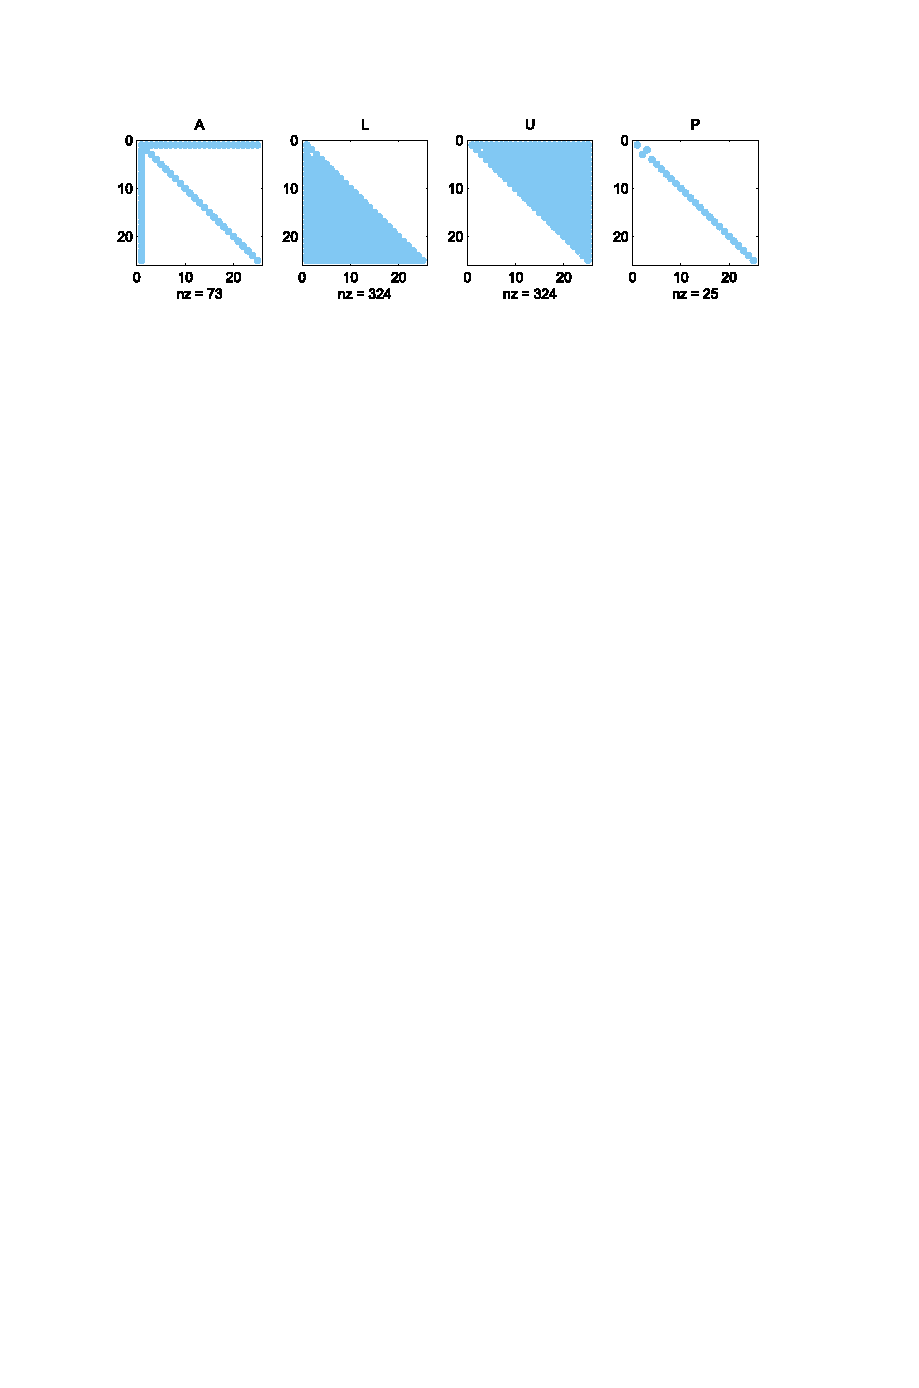
\includegraphics[width=\textwidth]{img/fill_in_1.pdf}
\end{examplebox}

\begin{examplebox}
    Un altro esempio di \emph{fill-in} su una generica matrice. In questo caso, gli elementi non nulli della prima riga e della prima colonna di $A$ inducono un riempimento totale delle corrispondenti colonne in $U$ e righe in $L$, rispettivamente, mentre gli elementi non nulli sopra e sotto le diagonali di $A$ comportano un riempimento delle diagonali superiori di $U$ ed inferiori di $L$ comprese tra quella principale e quelle non nulle di $A$.

    \highspace
    \centering
    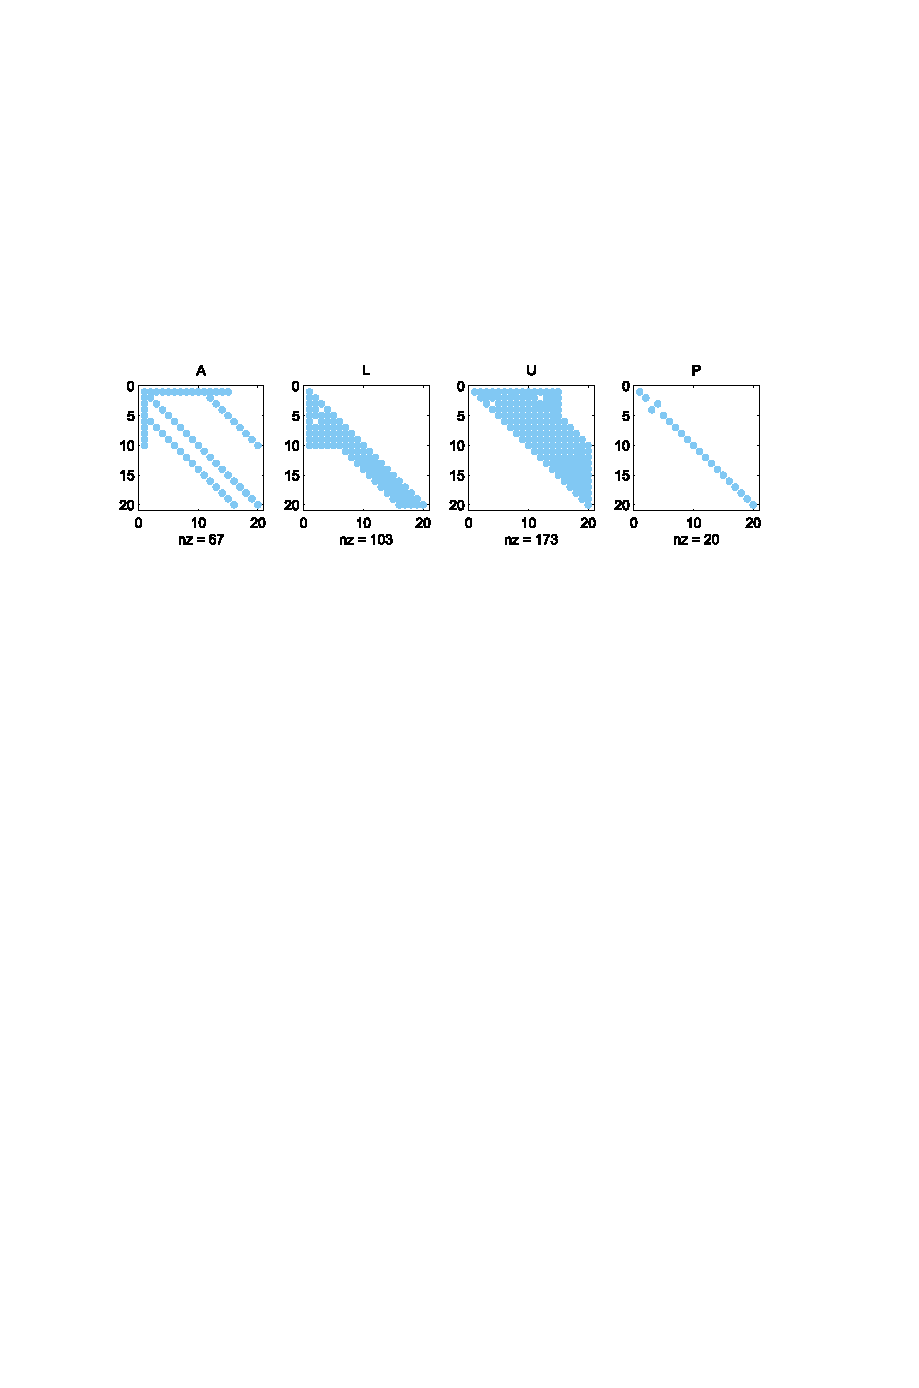
\includegraphics[width=\textwidth]{img/fill_in_2.pdf}
\end{examplebox}

\begin{flushleft}
    \textcolor{Green3}{\faIcon{question-circle} \textbf{Come risolvere il \emph{fill-in}?}}
\end{flushleft}
Per ovviare al problema del \emph{fill-in}, si possono adottare \textbf{tecniche di riordinamento che permutano righe e colonne della matrice prima di realizzare la fattorizzazione}. Tuttavia, in alcuni casi la \textbf{sola applicazione della tecnica di pivoting totale} (paragrafo \ref{subsubsection: Il pivoting totale} pagina \pageref{subsubsection: Il pivoting totale}) consente di raggiungere lo stesso obiettivo.

\highspace
Prima di introdurre un nuovo esempio, si forniscono due definizioni.

\begin{definitionbox}
    Una matrice quadrata di dimensione $n$ è detta \definition{matrice sparsa} se ha un numero di elementi non nulli dell'ordine di $n$ (e non di $n^{2}$).
\end{definitionbox}

\begin{definitionbox}
    Si chiama \definition{pattern} di una matrice sparsa l'insieme dei suoi elementi non nulli.
\end{definitionbox}

\begin{examplebox}
    Nella seguente figura sono mostrati i pattern delle matrici ottenute dalla fattorizzazione con pivotazione totale. Come si può vedere, il fenomeno di \emph{fill-in} è contenuto.

    \highspace
    \centering
    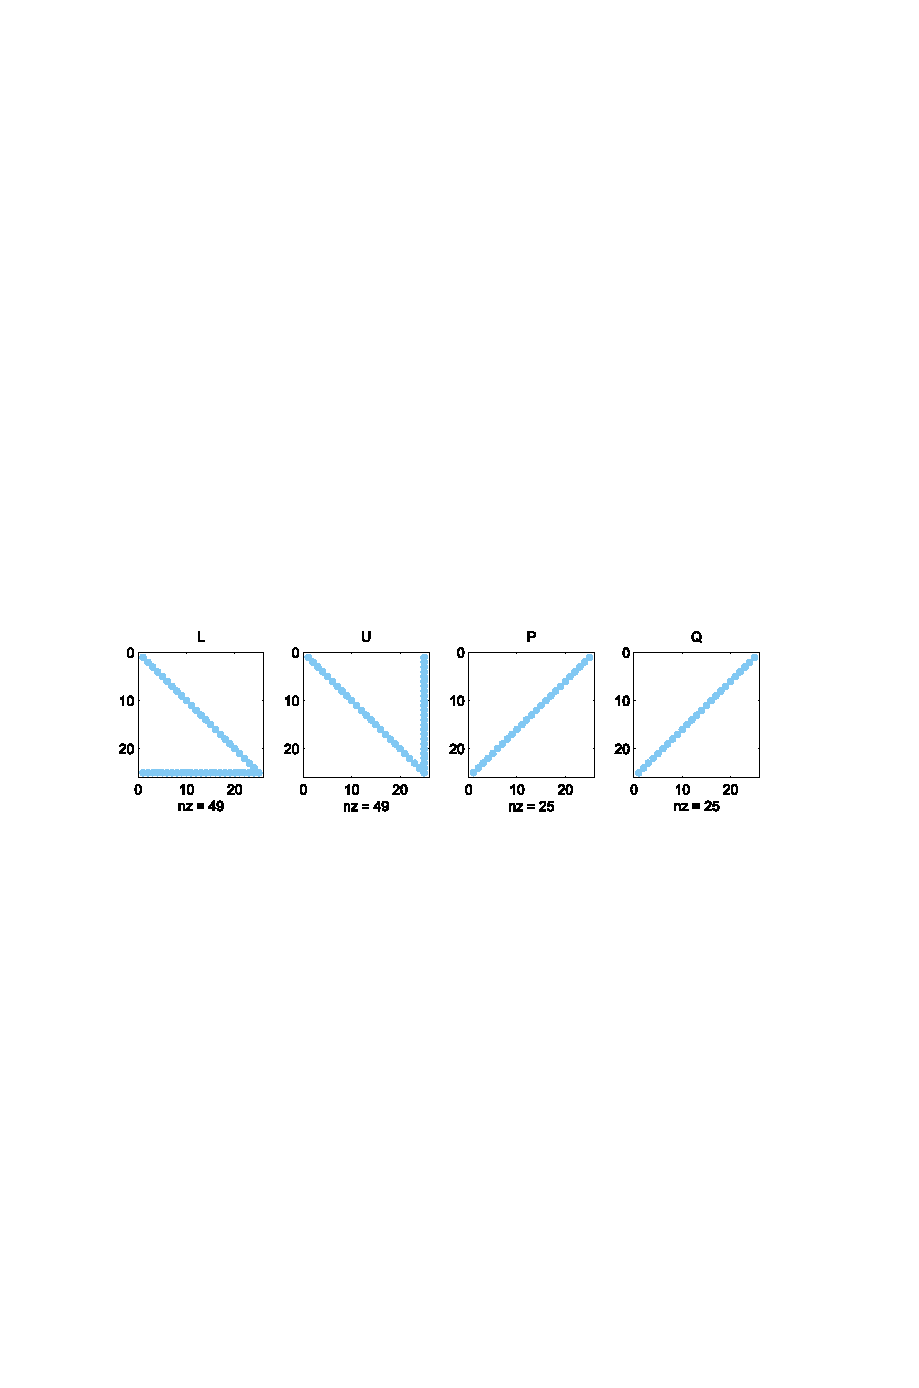
\includegraphics[width=\textwidth]{img/fill_in_3.pdf}

    \highspace
    Un altro esempio.

    \highspace
    \centering
    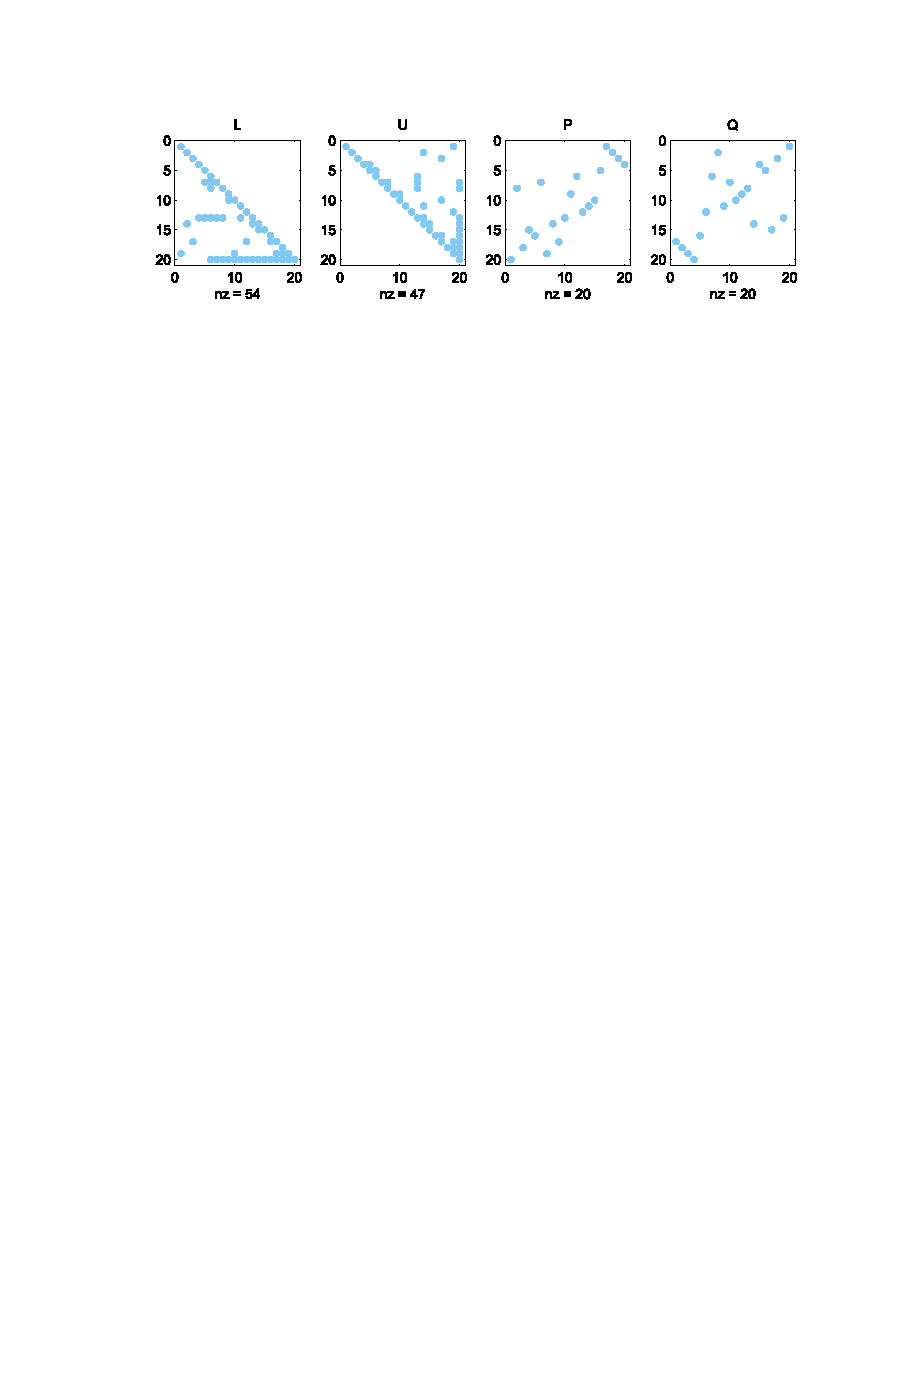
\includegraphics[width=\textwidth]{img/fill_in_4.pdf}
\end{examplebox}